\subsection{Boltzmann Machine}

% --- Lucas

\begin{figure}[htbp]
	\begin{center}
		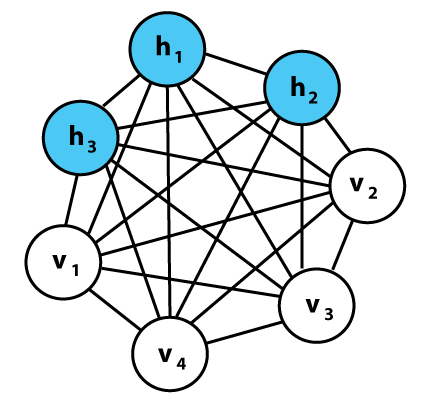
\includegraphics[width=0.5\textwidth]{inc/boltzmann_machine.png}
		\caption{Illustration of a Boltzmann Machine. The blue units represents three hidden units, while the four white units represents four visible units.\protect\footnotemark}
		\label{fig:boltzmann_machine}
	\end{center}
\end{figure}
\footnotetext{Original image (Public Domain): \url{https://en.wikipedia.org/wiki/File:Boltzmannexamplev1.png}}

The "Boltzmann Machine" (BM) is a form of "parallel constraint satisfaction network" \cite{ackley1985learning}. It is capable of learning the underlying constraints of a domain by only being shown examples of it. The BM is composed of units forming a complete graph where the connection between two units are symmetric, meaning that the weight on the connection is the same in either direction. No unit has a connection to itself. The units are binary, meaning that they can assume one of two states, on or off. The state of a unit is determined by a probabilistic function based on the states of the units neighbours. A strong connection (high weight value) between two units indicates that if either of these two units are active, the other one should probably be active as well. While a weak connection (low weight value) indicates that these should probably not be active at the same time.

The BM is notably similar to the Hopfield network in that it also defines a global energy state of the system, utilizing the same equation that determines the global energy value. Each global state can be identified by the energy of the system in that state. By forcing the values of the visible units to represent a training set the system attempts to find an energy configuration that is compatible with the given input. The resulting energy state can then be interpreted as to how well the given data fulfils the constraints of the domain. Thus by minimizing the energy the system learns an interpretation of the problem that increasingly satisfies the constraints of the domain.

The simplest way to minimize the energy into a local minimum of the system is to change each unit into a value that results in a lower energy state. The data needed to determine this change is locally accessible to each unit. If the sum of all values for a given units neighbour exceeds the threshold of that unit, the resulting state of the unit should be on. Otherwise it should be off. This is the usual algorithm for binary units.

Because of this deterministic algorithm it suffers from the usual weaknesses of gradient descent algorithms, namely it gets stuck in local minima if its initial state is close to one. In order to alleviate the algorithm of this problem noise is introduced in the training. This allows the network to "jump" out of these minima into configurations of higher energy. The algorithm used for noise introduction is a variation of the "Metropolis algorithm" \cite{metropolis1953equation} that was used to study thermodynamic systems. This modified version introduces a concept of temperature to the machine. The machine then tries to reach "thermal equilibrium" during training. Meaning that the machine is allowed to run repeatedly until the global energy of the system converges to a fixed state over a temperature that is initially high and then slowly decreased over the runtime of the system. The probability of finding the system in a global state after it has reached thermal equilibrium follows a Boltzmann distribution.

%TODO discuss the usage of hebbian learning in boltzmann
%TODO write more about this temperature thing
%TODO write more about the probabilistic features of the BM as well as the boltzmann distribution that gives the system its name.

Training is conducted in two phases, in the first phase the visible units of the machine are set to the values of the training set. In the next phase the machine is allowed to run freely, independent of the training set. The machine is iteratively switched between these two phases for the duration of the training until it reaches thermal equilibrium. The goal of the training is for the machine to generate the input vector with a high probability.

% --- NOTES
%The difference between the BM and the Hopfield network is mainly that the nodes (or units as they are referred to in the original paper) of the Boltzmann Machine are stochastic by nature.
%The BM can be used for constraint satisfaction problems that involve a large amount of weak constraints.
